% !TeX spellcheck = cs_CZ
%{\tikzset{external/prefix={tikz/CES/}}
% \tikzset{external/figure name/.add={ch08_}{}}
%---------------------------------------------------------------------------------------------------
% file STM32.tex
%---------------------------------------------------------------------------------------------------
%==============================Kapitola: Průvodce procesory rodiny STM32F4==========================
\setchaptertoc
\chapter{Průvodce procesory rodiny STM32F4}

Embedded systém (\texttt{zabudovaný systém}, \textbf{vestavěný system}), lze podle wikipedie 
charakterizovat jako jednoúčelový systém, ve kterém je řídicí počítač zcela zabudován do zařízení, 
které ovládá. Na rozdíl od univerzálních počítačů, jako jsou osobní počítače, jsou zabudované 
počítače většinou jednoúčelové (např. bankomat, kalkulačka, myčka nádobí, klimatizace, atd.), 
určené pro předem definované činnosti. Vzhledem k tomu, že systém je určen pro konkrétní účel, 
mohou tvůrci systém při návrhu optimalizovat pro konkrétní aplikaci, a tak snížit cenu výrobku. 
Vestavěné systémy jsou často vyráběny sériově ve velkém množství, takže úspora bývá znásobena 
velkým počtem vyrobených kusů.

Počítače do dlaně (PDA), mobilní digitální pomocníci (MDA) a inteligentní mobilní telefony 
(smartphone) jsou také často označovány jako vestavěná zařízení vzhledem k vlastnostem hardware i 
přes to, že z hlediska software jsou rozšiřitelné a všeobecně použitelné podobně jako osobní 
počítače. S rozvojem těchto zařízení se stírá hranice mezi vestavěnými zařízeními a osobními 
počítači.

\section{Vestavěné systémy s ARM procesory}
  Jádra procesoru ARM je klíčovou součástí mnoha úspěšných 32bitových vestavěných systémů 
  \cite[s.~3]{sloss2004arm}.
  
  \subsection{Filosofie RISC architektury}
  
  \subsection{Filosofie ARM architektury}
  \subsection{Embedded System Hardware}
  \subsection{Embedded System Software}

\section{Úvod do architektury ARM}
  Předchozí kapitola pojednávala obecně o vestavěných systémech. V této kapitole se zaměříme na 
  představení procesorového jádra ARM architektury a popíšeme tok dat mezi jednotlivými částmi 
  jádra. Na procesorové jádro se podíváme z programátorské perspektivy 
  
%  We will describe the programmer’s model from a software developer’s view of the ARM processor, 
%  which will show you the functions of the processor core and how different parts interact. We 
%will 
%  also take a look at the core extensions that form an ARM processor. Core extensions speed up and 
%  organize main memory as well as extend the instruction set. We will then cover the revisions to 
%  the ARM core architecture by describing the ARM core naming conventions used to identify
%  them and the chronological changes to the ARM instruction set architecture. The final section 
%  introduces the architecture implementations by subdividing them into specific ARM processor core 
%  families.
  
  \subsection{Registry}
  \subsection{Current Status Program Register}
  \subsection{Pipeline}
  \subsection{Výjimky, přerušení a tabulka vektorů}
  \subsection{Rozšíření jádra}
  \subsection{Revize architektury}
  \subsection{Rodiny ARM }


\section{Architektura mikroprocesoru STM32F100xx}
  Jádro Cortex-M3 je založeno na Harvardské architektuře (kap. \ref{ces:IchapIVsecIssecIII}), která 
  má oddělenou sběrnici pro data a pro instrukce. To umožňuje rychlejší vykonávání programového 
  kódu, kdy je možné paralelně načítat novou instrukci a zároveň ukládat data výsledku do paměti. 
  Toho se využívá při pipeliningu (zřetězování instrukcí nebo průtokové zpracování instrukcí[5]), 
  který má 3 fáze - načtení instrukce, dekódování instrukce a vykonání instrukce. Zároveň se také 
  odhaduje, zda může aktuálně vykonávaná instrukce větvení ovlivnit aktuálně načítanou a 
  dekódovanou instrukci. Mechanismus pipeliningu tím umožňuje mnohonásobné zvětšení výkonu vzhledem 
  k hodinovému kmitočtu jádra mikrokontroléru.  
  \begin{figure}[ht!] %\ref{MIT:fig_stm32f100arch}
    \centering
    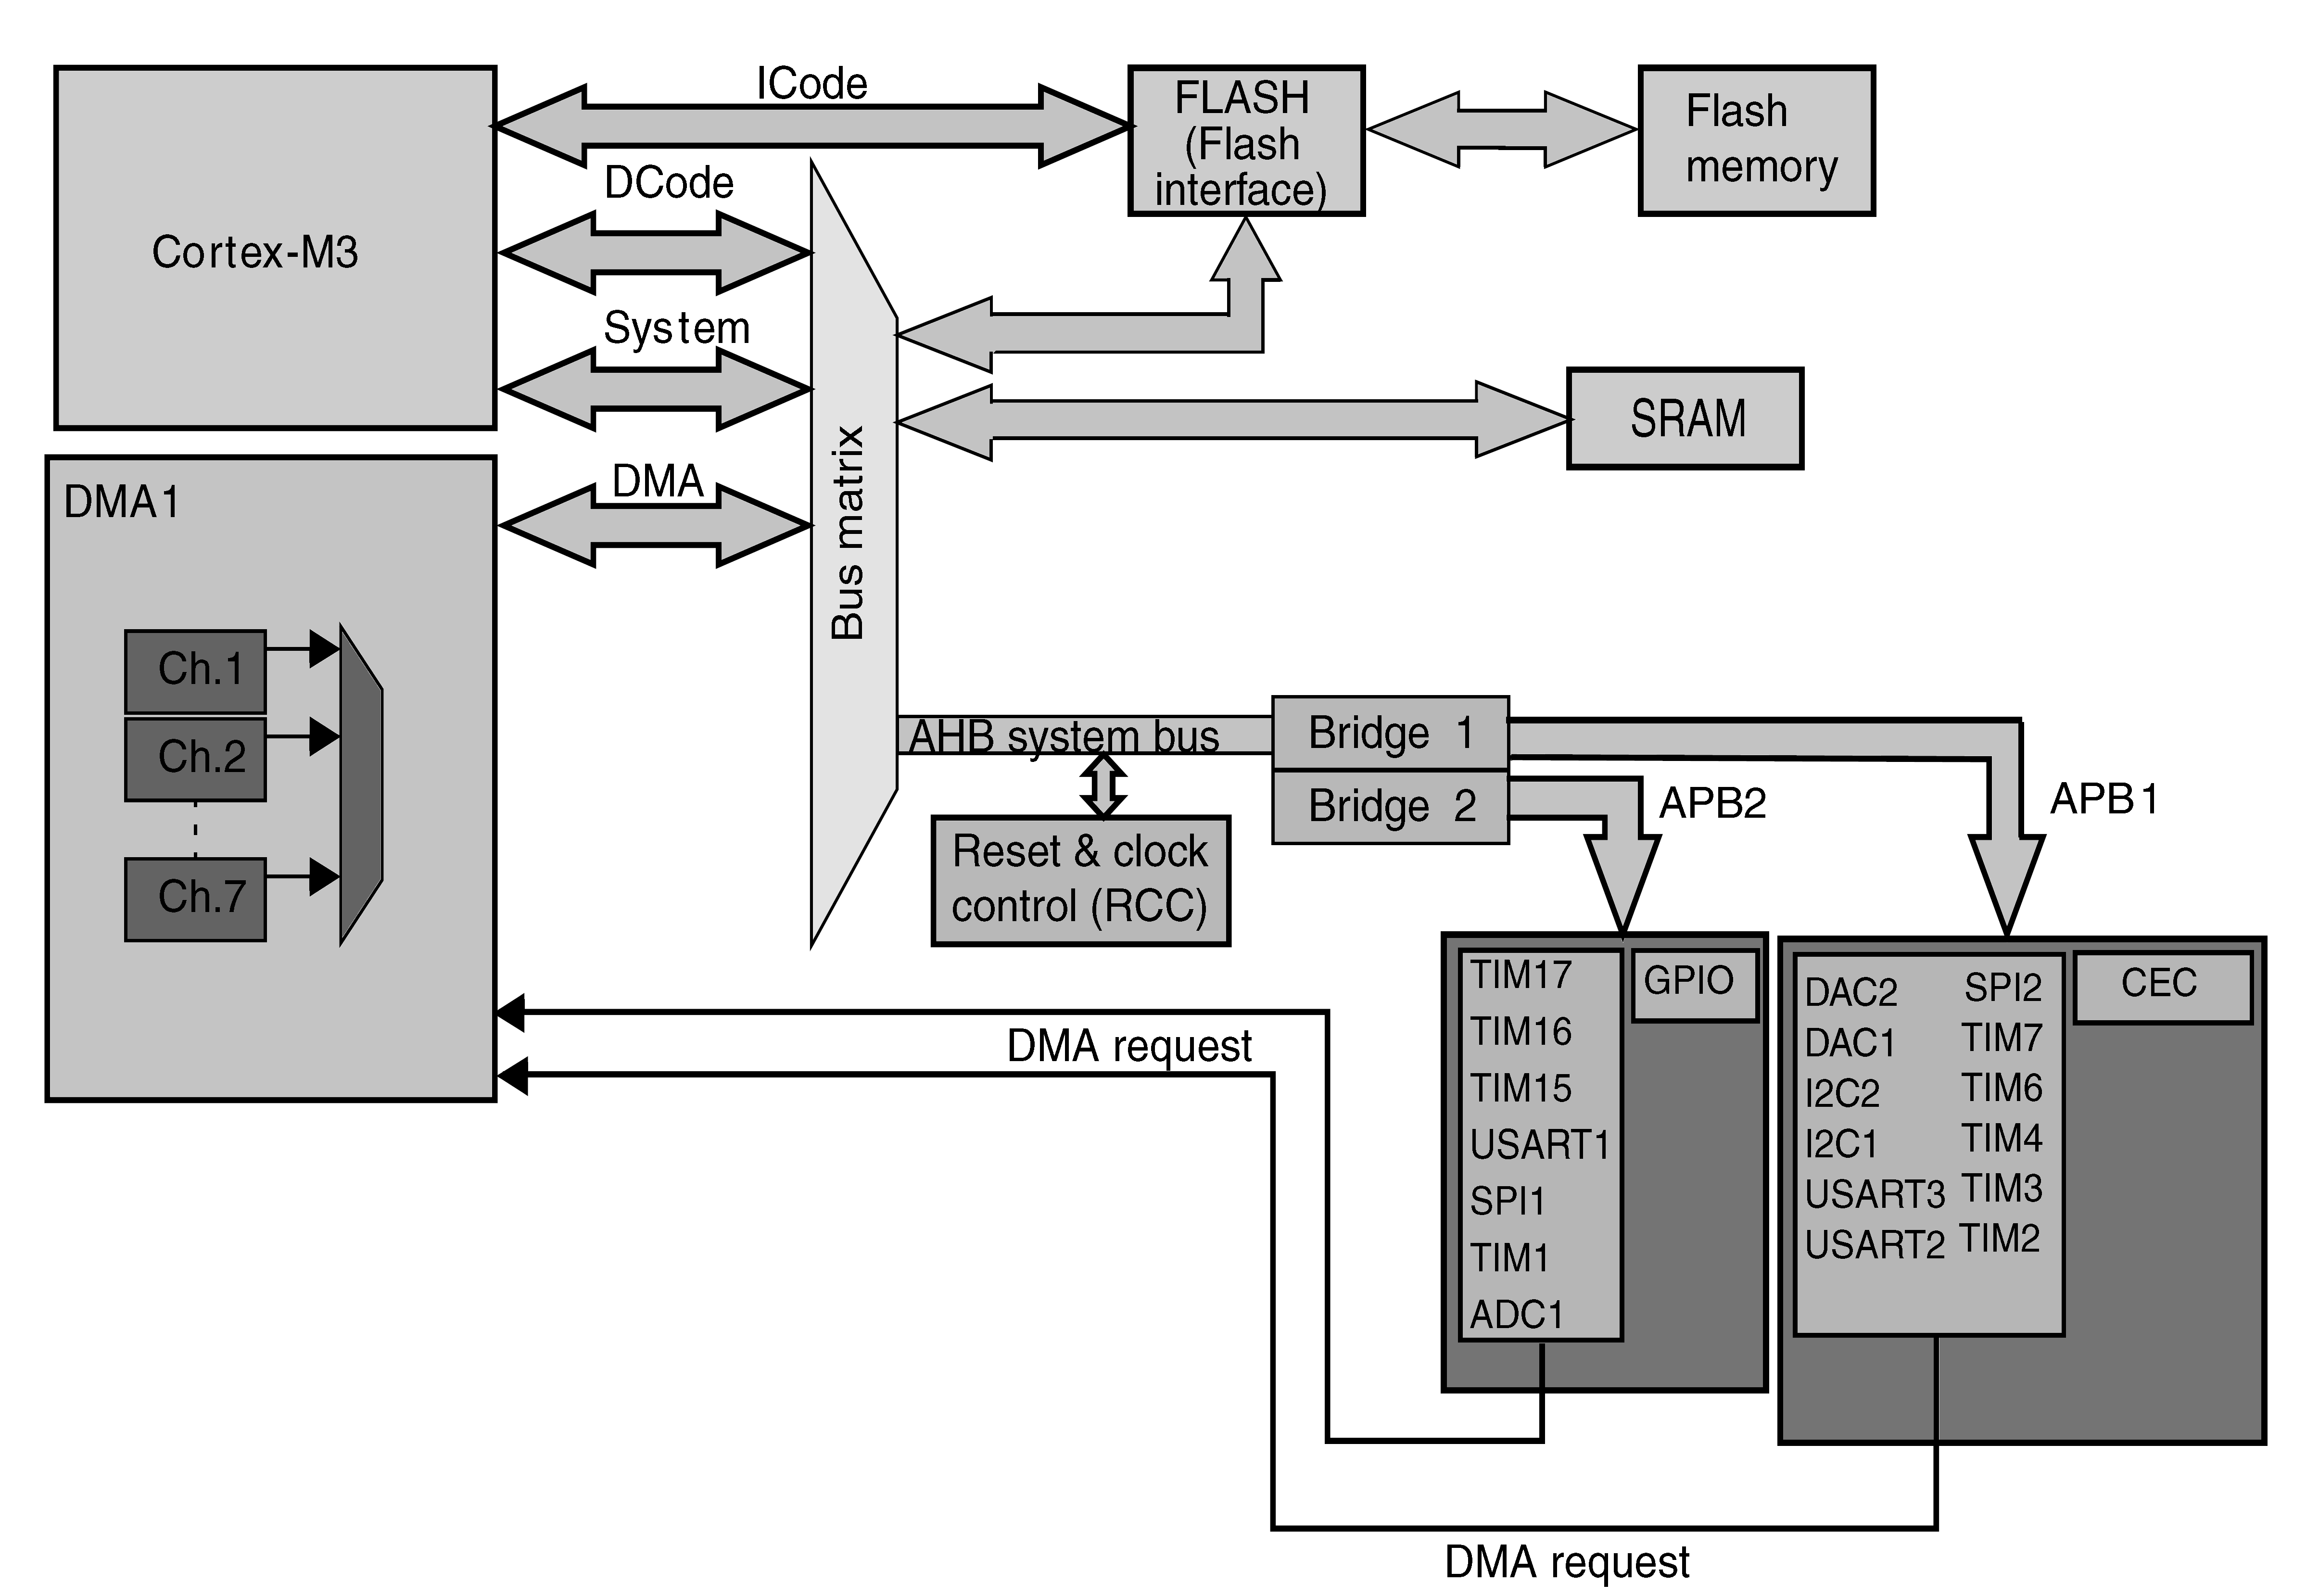
\includegraphics[width=1\linewidth]{STM32F100_arch.png}
    \caption{Architektura systému nízké a střední hustoty řady Value Line}
    \label{MIT:fig_stm32f100arch}
  \end{figure}
  
  \subsection{Reset and clock control (RCC)}
  \subsection{GPIO}
  
  \begin{figure}[ht!] %\ref{CES:fig002}
    \centering
    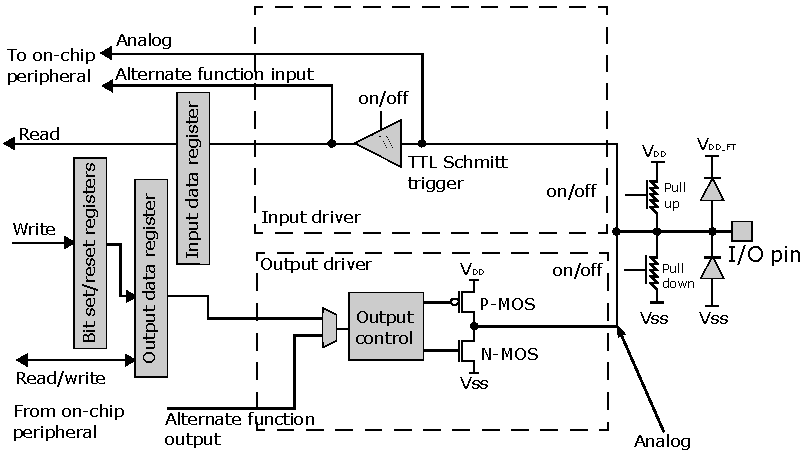
\includegraphics[width=1\linewidth]{ces_fig002.pdf}
    \caption{xxx}
    \label{CES:fig002}
  \end{figure}
   


  \begin{itemize}
    \item \href{http://librarian/stable.php?id=141}{CMSIS Tutorial}
  \end{itemize}
  

\section{Přístupy k programování ARM}
\begin{description}
  \item[CMSIS] Programování pouze s knihovnou CMSIS se velice podobá programovacím stylům 
    8bitových mikrokontrolérů. Programujete tím stylem, že přímo zapisujete a čtete z registrů 
    (SFR). Vystačíme si s hlavičkovým souborem, který obsahuje stovky maker a definic    
    usnadňujících vám přístup k řídicím registrům čipu.
  
    Během programování je nezbytně nutné stále nahlížet do datasheetu na funkci jednotlivých bitů v 
    registrech. Je to tedy velice pracná a zdlouhavá metoda. Jedinou její výhodou (a to velice 
    spornou) je fakt, že se nemusíte učit, jak pracují knihovní funkce. Využitelná je v aplikacích, 
    které jsou úzce vázané na periferie čipu. Tedy v aplikacích zaměřených primárně na hardware.
  \item[SPL] Programování s pomocí knihoven SPL (\emph{Standard Peripheral Library}) je postup, 
    který nemá budoucnost, protože podpora SPL byla před více než rokem ukončena. Ke starším čipům, 
    jako třeba STM32F407 (a mnoha dalším), jsou SPL k dispozici. Pokud ale začínáte, je pro vás 
    výhodnější učit se knihovny LL nebo HAL.
  \item [LL API] Nízkoúrovňové (Low Level) knihovny slouží pro kompletní ovládání periferií. 
    Odstiňují vás od přímé práce s registry, aniž by ale obětovaly některé z funkcí periferií. 
    Jejich blízký vztah k periferiím snižuje teoreticky přenositelnost programu. Na druhou stranu 
    umožňuje plně rozvinout schopnosti periferií. Jim se budu ve svém tutoriálu věnovat.
  \item [HAL API] Vysokoúrovňové knihovny (High Abstraction Layer) jsou dobře přenositelné. 
    Odstiňují programátora od detailní práce s periferiemi. Díky tomu je konfigurace periferií 
    rychlejší. 
\end{description}


\section{CMSIS}
  \begin{itemize}
    \item \href{http://librarian/stable.php?id=141}{CMSIS Tutorial}
  \end{itemize}
  
%} % tikzset
%---------------------------------------------------------------------------------------------------